\section{Paper C: Hybrid LSMC-PDE for GDMR}

\begin{frame}{Paper C: Hybrid LSMC-PDE under GDMR}
  \begin{columns}[T,onlytextwidth]
    \begin{column}{0.50\textwidth}
      \begin{block}{GDMR model}
        {\scriptsize
        \[
        \begin{aligned}
        \dd S_t &= rS_t\dd t+S_t\sqrt{v_t}\dd W_t^{(1)},\\
        \dd v_t &= \kappa_1(v'_t-v_t)\dd t+\xi_1v_t^{\delta_1}\dd W_t^{(2)},\\
        \dd v'_t &= \kappa_2(\theta-v'_t)\dd t+\xi_2(v'_t)^{\delta_2}\dd W_t^{(3)}.
        \end{aligned}
        \]}
        {\small The variance equations do not involve \(S_t\). This one-way coupling is the main structure used by the hybrid method.}
      \end{block}
    \end{column}
    \begin{column}{0.46\textwidth}
      \begin{block}{Plain LSMC}
        The continuation value is regressed on the full state: asset level \(S\), current variance \(v\), and long-run variance \(w=v'\).
      \end{block}
      \begin{block}{Hybrid LSMC-PDE}
        Simulate \((v,w)\), handle the stock-price direction on a log-price grid by conditional FFT/PDE, and regress only over \((v,w)\).
      \end{block}
    \end{column}
  \end{columns}

  \vspace{0.35em}
  \keymessage{The goal is not to change the Bermudan recursion; it is to make the continuation-value approximation easier.}
\end{frame}

\begin{frame}{Paper C: Hybrid Decomposition of the Continuation Value}
  \vspace{-0.35em}
  {\scriptsize
  \[
  U_M(s,v,w)=h_M(s),\qquad
  U_n(s,v,w)=\max\{h_n(s),C_n(s,v,w)\}.
  \]
  \[
  C_n(s,v,w)=e^{-r\Delta t_n}
  \E\!\left[
  U_{n+1}(S_{t_{n+1}},v_{t_{n+1}},v'_{t_{n+1}})
  \mid S_{t_n}=s,\;v_{t_n}=v,\;v'_{t_n}=w
  \right].
  \]
  }
  \vspace{-0.25em}
  \begin{columns}[T,onlytextwidth]
    \begin{column}{0.48\textwidth}
      \begin{block}{1. Inner conditional step}
        {\scriptsize
        Simulate the variance Brownian drivers over \([t_n,t_{n+1}]\) and condition on the enlarged information \(H_n\). The variance segment and the correlated part of the asset Brownian motion are then fixed, leaving only the orthogonal asset Brownian component:
        \[
        \resizebox{0.98\linewidth}{!}{$
        \bar C_n^F(s;H_n)=e^{-r\Delta t_n}
        \E\!\left[
        F(S_{t_{n+1}},v_{t_{n+1}},v'_{t_{n+1}})
        \mid S_{t_n}=s,\;H_n
        \right].
        $}
        \]
        }
      \end{block}
    \end{column}
    \begin{column}{0.48\textwidth}
      \begin{block}{2. Outer regression step}
        {\scriptsize
        The true continuation value is recovered by averaging the pathwise conditional surface over the current variance state:
        \[
        C_n^F(s,v,w)=
        \E\!\left[\bar C_n^F(s;H_n)
        \mid v_{t_n}=v,\;v'_{t_n}=w\right].
        \]
        In the algorithm, this outer expectation is approximated by least-squares regression over \((v,w)\), while \(s\) is carried by the log-price grid.}
      \end{block}
    \end{column}
  \end{columns}
  \vspace{0.15em}
  \keymessage{\footnotesize The hybrid split changes where approximation happens: PDE/FFT handles the stock-price direction path by path, and regression handles only the variance-state dependence.}
\end{frame}

\begin{frame}{Paper C: Hybrid LSMC-PDE Algorithm}
  \begin{columns}[T,onlytextwidth]
    \begin{column}{0.48\textwidth}
      \begin{block}{1. Brownian projection}
        {\scriptsize
        \[
          \dd W_t^{(1)}=\beta_2\dd W_t^{(2)}+\beta_3\dd W_t^{(3)}+\sigma_\perp\dd B_t^\perp .
        \]}
        Conditioning on the variance Brownian drivers leaves only the residual Brownian motion \(B^\perp\) in the asset direction.
      \end{block}
      \begin{block}{2. Path statistics}
        {\scriptsize
        \[
        \begin{aligned}
        Z_n^j&=\sum \sqrt{\bar v_\ell^j}(\beta_2\Delta W_\ell^{(2),j}+\beta_3\Delta W_\ell^{(3),j}),\\
        I_n^j&=\sum (r-\tfrac12\bar v_\ell^j)\Delta\tau_\ell,\qquad
        B_n^j=\sigma_\perp^2\sum \bar v_\ell^j\Delta\tau_\ell .
        \end{aligned}
        \]}
      \end{block}
    \end{column}
    \begin{column}{0.48\textwidth}
      \begin{block}{3. Conditional FFT step}
        {\scriptsize
        \[
        u_n^j\approx\operatorname{FFT}^{-1}\!\left(
        \operatorname{FFT}[g_{n+1}^j]
        \exp\{i\omega Z_n^j+i\omega I_n^j-\tfrac12\omega^2B_n^j\}
        \right).
        \]}
        The terminal grid is not shifted first; the shift enters through the Fourier multiplier.
      \end{block}
      \begin{block}{4. Regression over variance variables}
        {\scriptsize
        \[
        \widehat C_n^N(s_i,v,w)=a_n^N(s_i)\cdot\phi(v,w),\qquad w=v'.
        \]}
        The asset coordinate is carried by the grid \(s_i\); the regression learns only \((v,w)\).
      \end{block}
    \end{column}
  \end{columns}
\end{frame}

\begin{frame}{Paper C: Backward Hybrid Recursion}
  \begin{columns}[T,onlytextwidth]
    \begin{column}{0.54\textwidth}
      \begin{block}{Backward loop}
        \begin{enumerate}
          \item Initialize \(\widehat V_M^N(s_i,v,w)=h_M(s_i)\).
          \item For \(n=M-1,\ldots,1\), compute pathwise pre-surfaces \(\widehat C_n^j(s_i)\) using the FFT step.
          \item At each \(s_i\), regress \(\widehat C_n^j(s_i)\) on \(\phi(v_n^j,w_n^j)\).
          \item Set
          \[
            \widehat V_n^N(s_i,v,w)=\max\{h_n(s_i),\widehat C_n^N(s_i,v,w)\}.
          \]
        \end{enumerate}
      \end{block}
    \end{column}
    \begin{column}{0.40\textwidth}
      \begin{block}{Time zero}
        No regression is needed at \(t_0\). Average the first-step pre-surfaces:
        {\small
        \[
          \widehat C_0^N(s_i)=\frac1N\sum_{j=1}^N\widehat C_0^j(s_i).
        \]}
        Then interpolate at \(S_0\) and compute
        {\small
        \[
          \widehat V_0^N(S_0)=\max\{h_0(S_0),\widehat C_0^N(S_0)\}.
        \]}
      \end{block}
    \end{column}
  \end{columns}
\end{frame}

\begin{frame}{Paper C: Path-Budget Sensitivity}
  \begin{columns}[T,onlytextwidth]
    \begin{column}{0.68\textwidth}
      \centering
      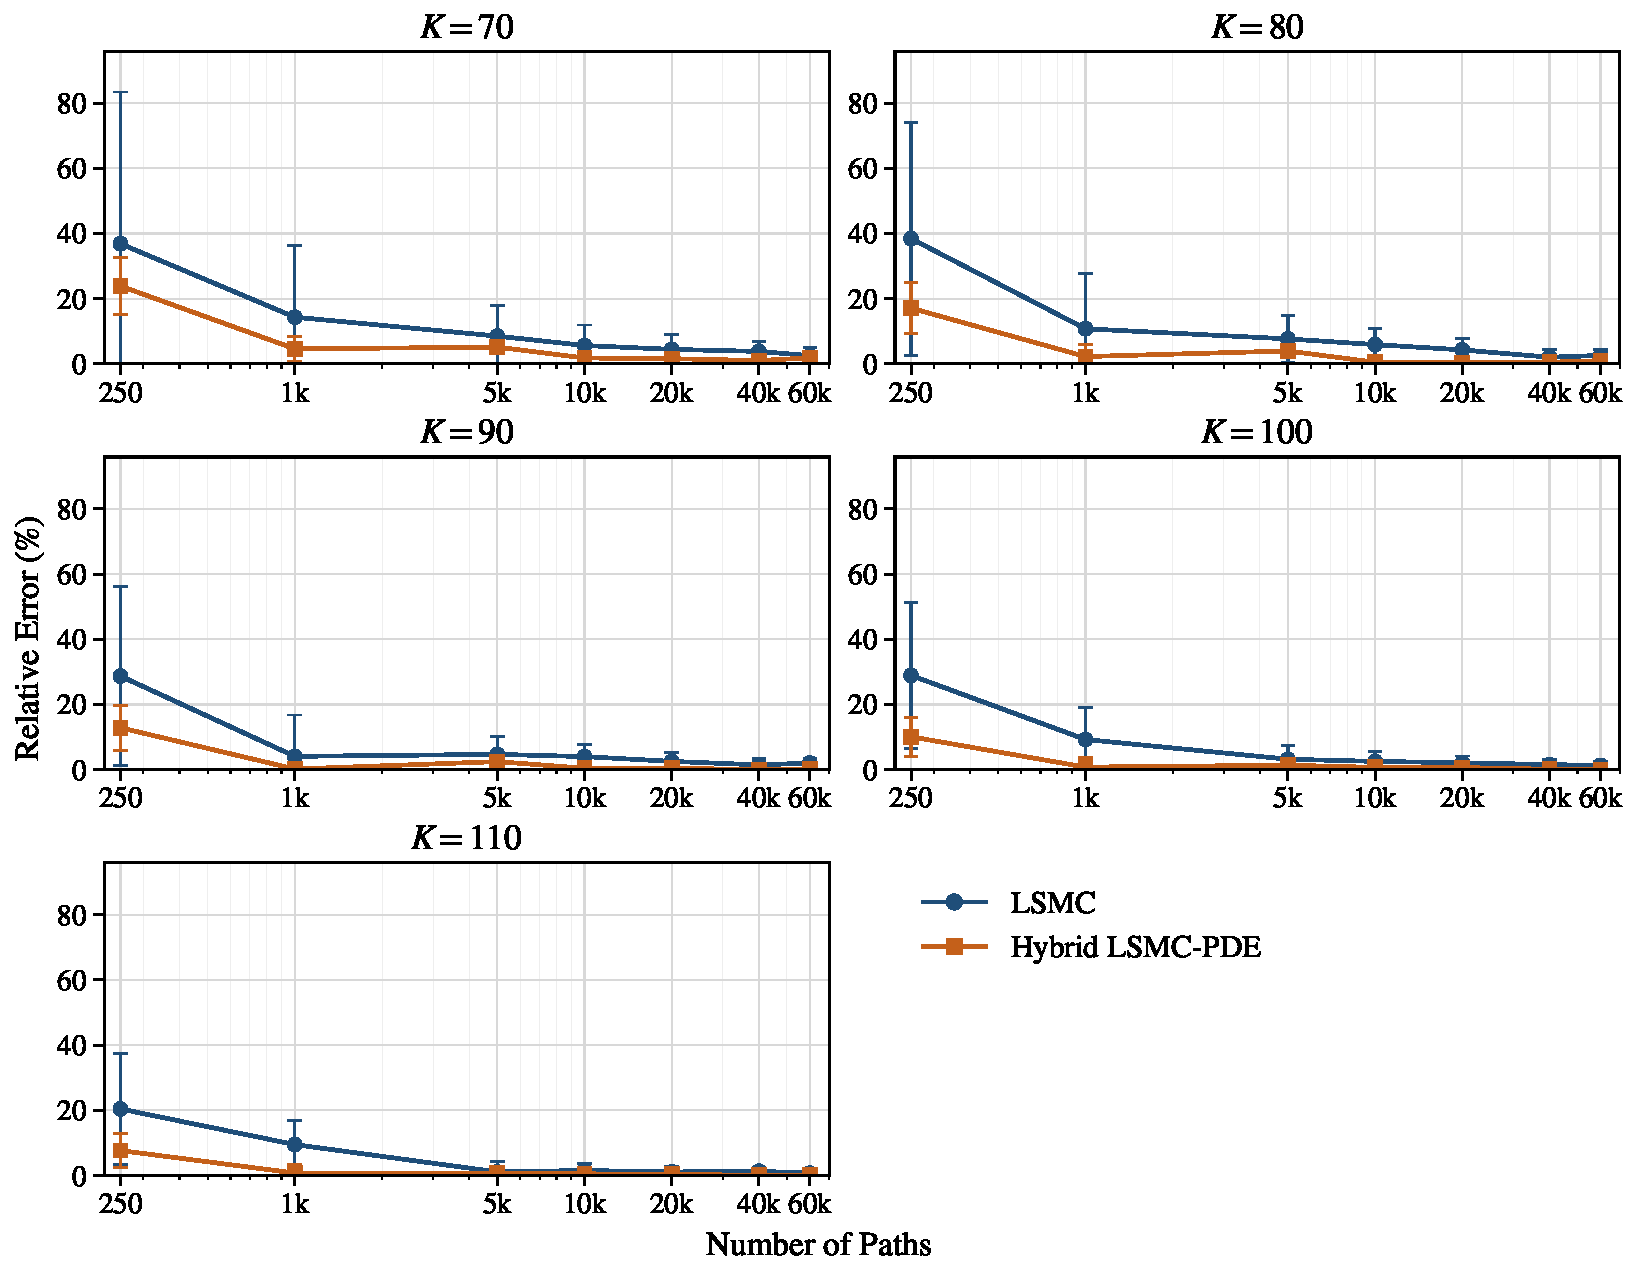
\includegraphics[width=\linewidth,height=0.72\textheight,keepaspectratio]{../Figures/PaperC/path_sweep_steps60_direct_relative_error.pdf}
    \end{column}
    \begin{column}{0.28\textwidth}
      \begin{block}{Interpretation}
        At fixed 60 Euler steps, the Hybrid LSMC-PDE estimator gives visibly lower relative errors in the low- and moderate-path regimes. 
      \end{block}
    \end{column}
  \end{columns}
\end{frame}

\begin{frame}{Paper C: Path-Budget Sensitivity at 48 Euler Steps}
  \begin{columns}[T,onlytextwidth]
    \begin{column}{0.68\textwidth}
      \centering
      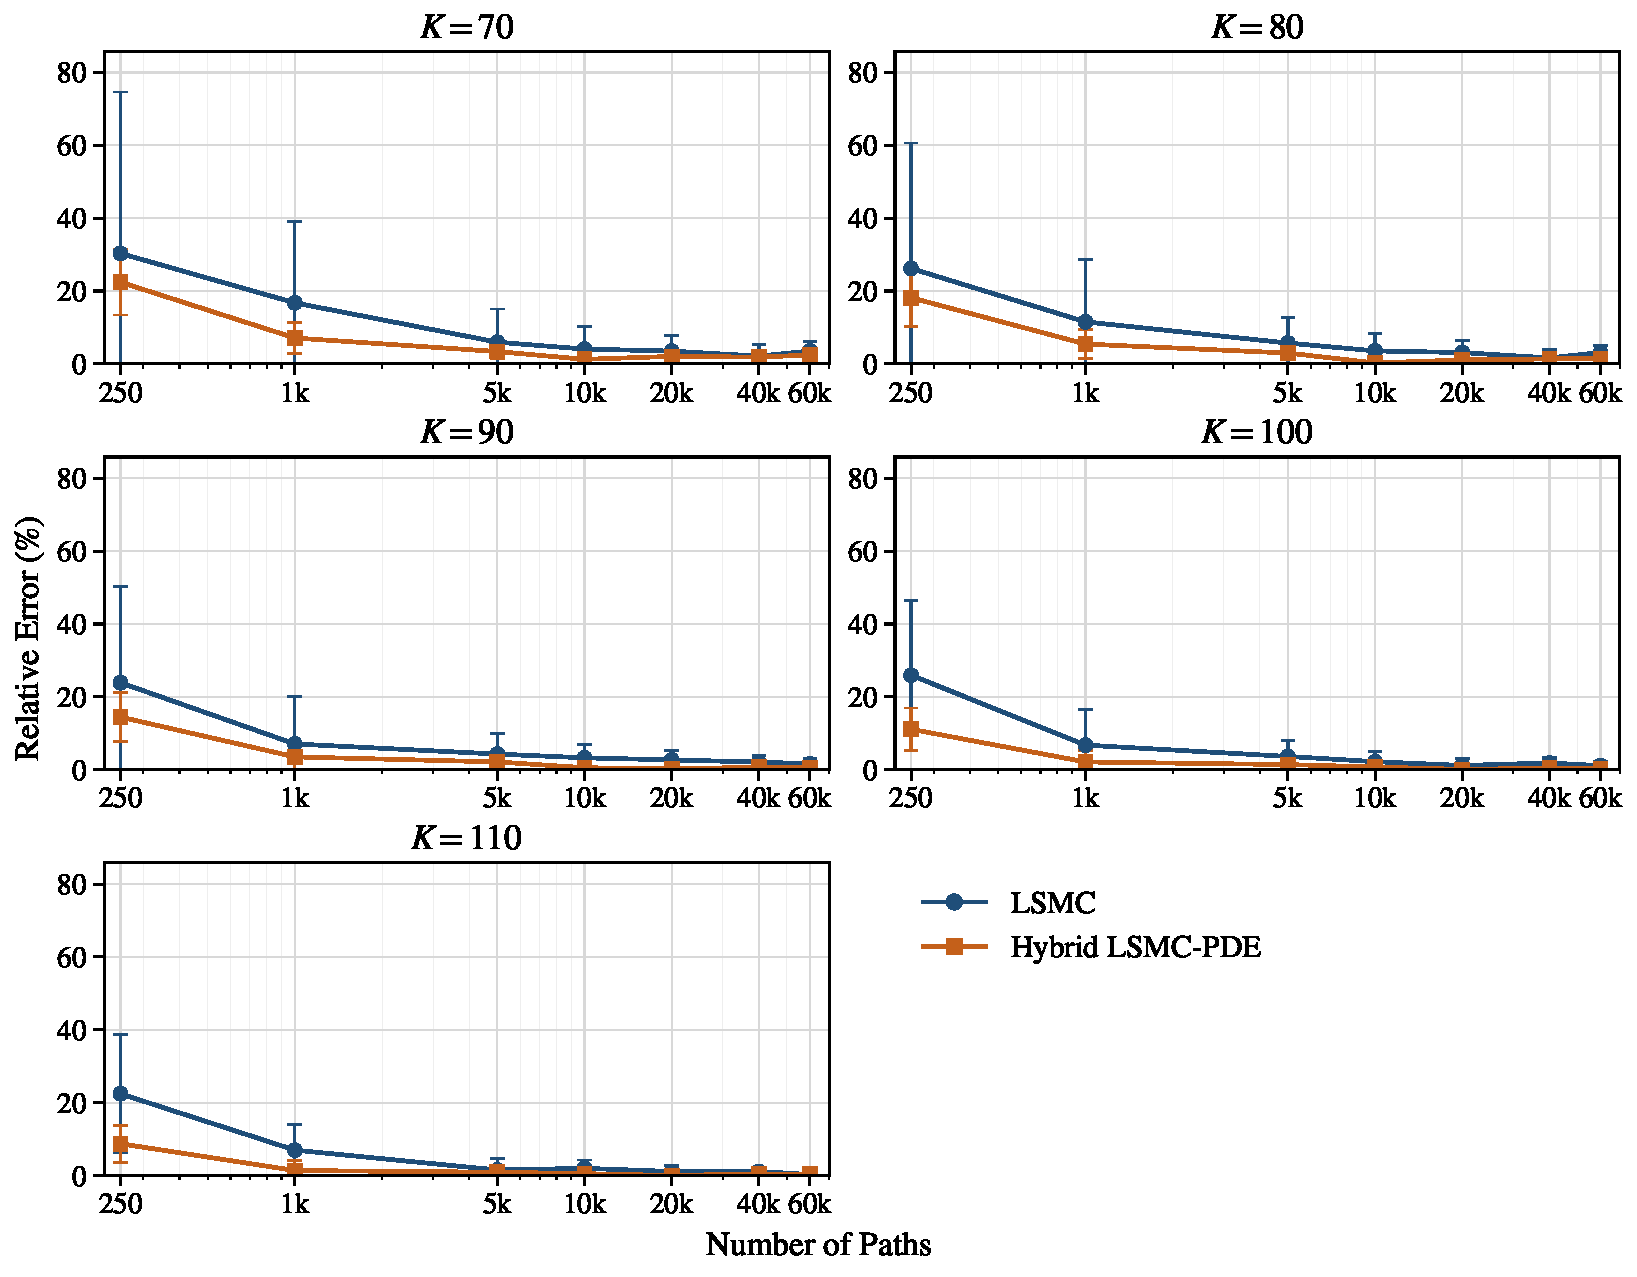
\includegraphics[width=\linewidth,height=0.72\textheight,keepaspectratio]{../Figures/PaperC/path_sweep_steps48_direct_relative_error.pdf}
    \end{column}
    \begin{column}{0.28\textwidth}
      \begin{block}{Interpretation}
        The 48-step experiment shows the same pattern: the hybrid estimator is most useful when the path budget is small or moderate. 
      \end{block}
    \end{column}
  \end{columns}
\end{frame}

\begin{frame}{Paper C: Time-Step Sensitivity}
  \begin{columns}[T,onlytextwidth]
    \begin{column}{0.68\textwidth}
      \centering
      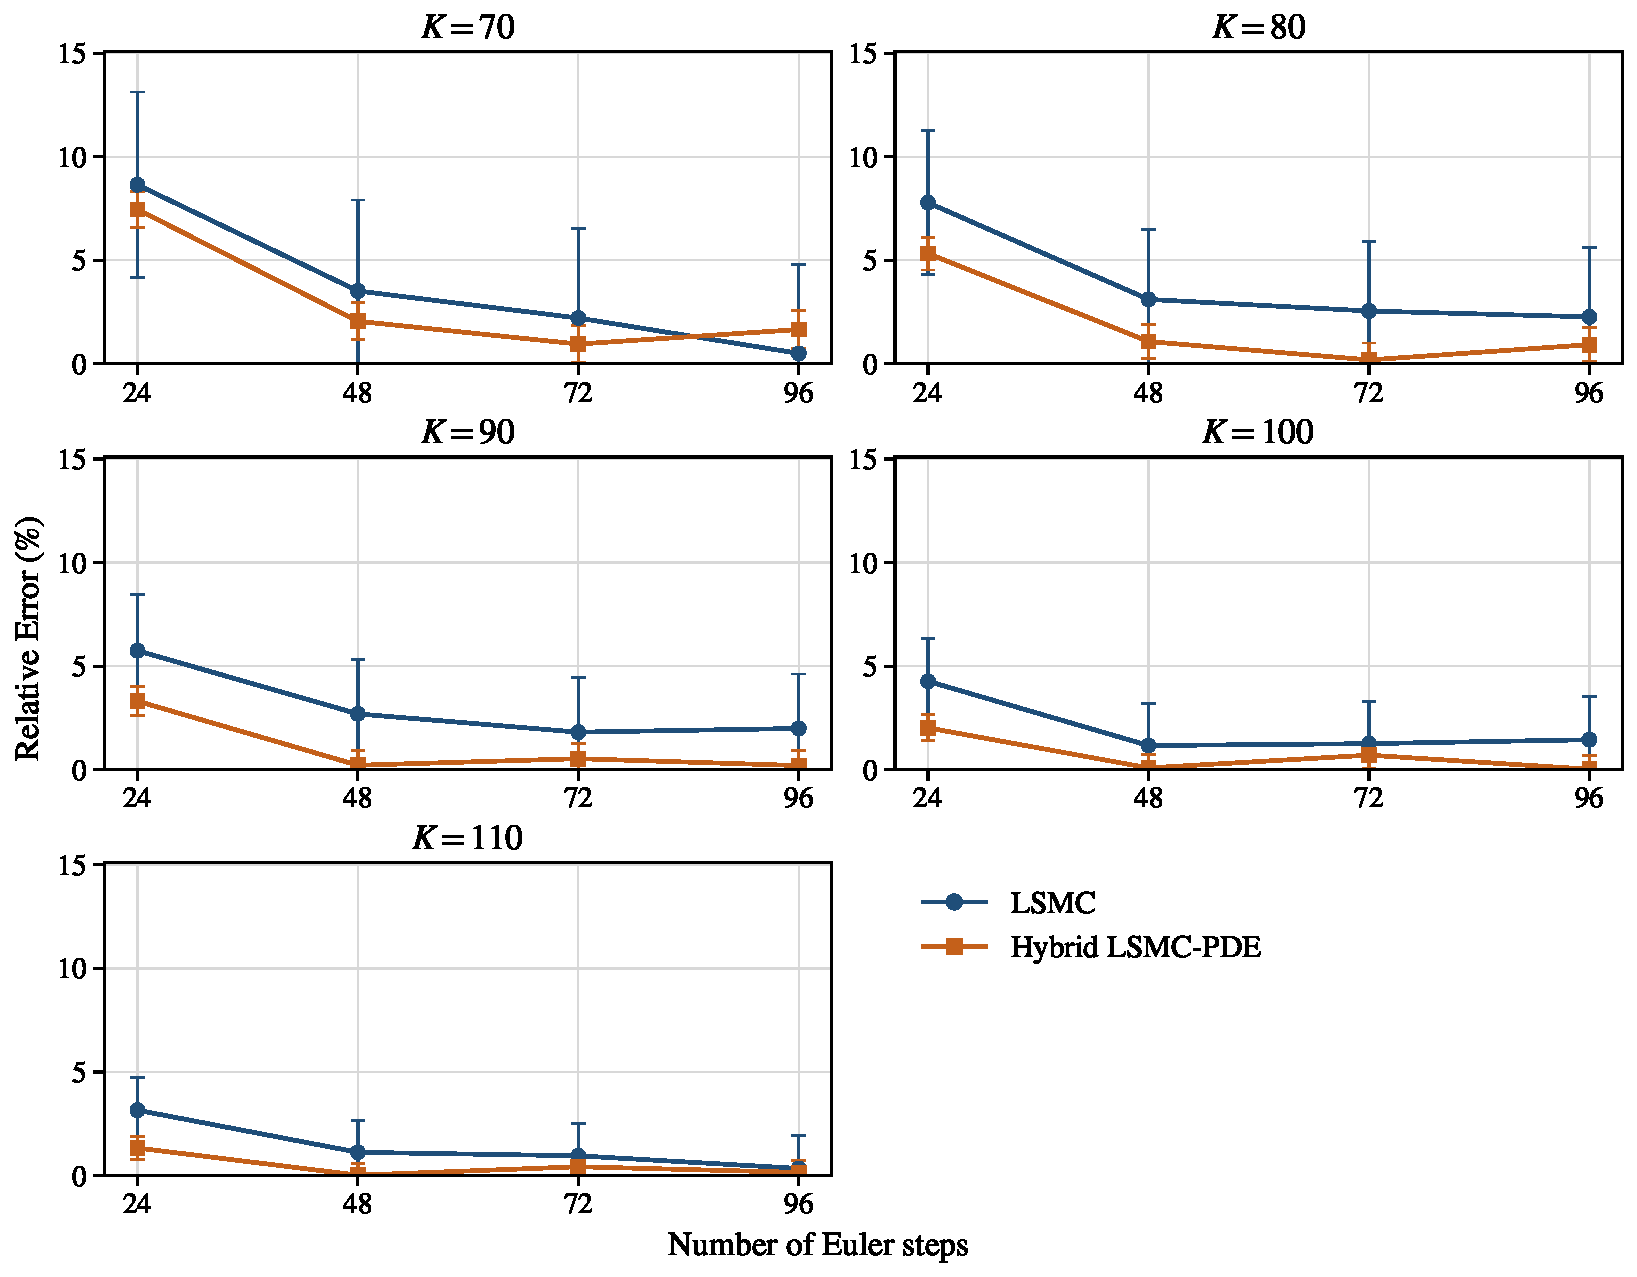
\includegraphics[width=\linewidth,height=0.72\textheight,keepaspectratio]{../Figures/PaperC/step_sweep_20k_direct_relative_error.pdf}
    \end{column}
    \begin{column}{0.28\textwidth}
      \begin{block}{Interpretation}
        With \(20{,}000\) paths, the Hybrid LSMC-PDE estimator is usually centered at lower relative errors across the tested Euler step counts. The conditional PDE step reduces the dimension of the continuation regression.
      \end{block}
    \end{column}
  \end{columns}
\end{frame}
